% !TEX root = ../main.tex
\chapter{Model Selection and Learning Theory}
\label{ch:selection}

\begin{intuition}[title=\textbf{Choosing the Right Model}]
A model that is too simple underfits; one that is too complex overfits. Model selection provides principled tools---information criteria, cross-validation, hyperparameter search, and theoretical bounds---for navigating this trade-off. Learning theory tells us \emph{why} generalisation is possible and how much data we need.
\end{intuition}

%% ----------------------------------------------------------------
\section{Information Criteria}

\begin{definition}[Akaike Information Criterion]
For a model with $d$ parameters and maximised log-likelihood $\hat\ell$:
\[
  \text{AIC} = -2\hat\ell + 2d.
\]
AIC estimates the expected KL divergence between the fitted model and the true distribution, up to a constant. Lower is better.
\end{definition}

\begin{definition}[Bayesian Information Criterion]
\[
  \text{BIC} = -2\hat\ell + d\ln n.
\]
BIC approximates the log of the marginal likelihood $p(\mathcal{D}\mid\mathcal{M})$ (Laplace approximation). It penalises complexity more heavily than AIC for $n\geq 8$.
\end{definition}

\begin{proposition}[BIC Derivation]
Starting from the Laplace approximation to the marginal likelihood:
\[
  p(\mathcal{D}\mid\mathcal{M}) \approx p(\mathcal{D}\mid\hat{\bm{\theta}})\,p(\hat{\bm{\theta}})\,(2\pi)^{d/2}\,|\bm{H}|^{-1/2},
\]
where $\bm{H}=-\nabla^2\ln p(\mathcal{D}\mid\bm{\theta})\big|_{\hat{\bm{\theta}}}$ is the observed Fisher information. Taking logarithms and noting that $\bm{H}=O(n)$ element-wise, we get
\[
  \ln p(\mathcal{D}\mid\mathcal{M}) \approx \hat\ell - \frac{d}{2}\ln n + O(1),
\]
whence $\text{BIC}\approx -2\ln p(\mathcal{D}\mid\mathcal{M})$ up to constants independent of the model.
\end{proposition}

\begin{bestpractice}[title=\textbf{AIC vs BIC in Practice}]
\begin{itemize}
  \item \textbf{AIC}: asymptotically optimal for \emph{prediction}; tends to select larger models.
  \item \textbf{BIC}: consistent for \emph{model identification} (selects the true model as $n\to\infty$); tends to select smaller models.
  \item When in doubt, use cross-validation, which makes no distributional assumptions.
\end{itemize}
\end{bestpractice}

%% ----------------------------------------------------------------
\section{Hyperparameter Tuning}

\begin{definition}[Hyperparameter Optimisation]
Given a model $\mathcal{M}_\lambda$ parameterised by hyperparameters $\lambda\in\Lambda$, we seek
\[
  \lambda^* = \argmin_{\lambda\in\Lambda}\; \hat{R}_{\text{CV}}(\lambda),
\]
where $\hat{R}_{\text{CV}}$ is the cross-validated risk estimate.
\end{definition}

\subsection{Grid Search}

\begin{algorithme}[title=\textbf{Grid Search}]
Define a grid $\Lambda_{\text{grid}}=\Lambda_1\times\Lambda_2\times\cdots\times\Lambda_m$ over $m$ hyperparameters. Evaluate $\hat{R}_{\text{CV}}(\lambda)$ for every $\lambda\in\Lambda_{\text{grid}}$ and return the minimiser.

\medskip
\textbf{Complexity:} $|\Lambda_{\text{grid}}|=\prod_{j=1}^m |\Lambda_j|$. The cost grows \emph{exponentially} in $m$.
\end{algorithme}

\subsection{Random Search}

\begin{theorem}[Efficiency of Random Search (Bergstra \& Bengio, 2012)]
If only $d_{\text{eff}}$ out of $m$ hyperparameters significantly affect performance, random search finds a near-optimal configuration with probability $1-\delta$ in
\[
  N = \lceil (1/\epsilon)^{d_{\text{eff}}}\,\ln(1/\delta) \rceil
\]
trials, independently of the remaining $m-d_{\text{eff}}$ irrelevant dimensions. Grid search, by contrast, wastes budget evaluating many redundant combinations.
\end{theorem}

\subsection{Bayesian Optimisation}

\begin{algorithme}[title=\textbf{Bayesian Hyperparameter Optimisation}]
\begin{enumerate}
  \item Place a GP prior on the objective $f(\lambda)=\hat R_{\text{CV}}(\lambda)$.
  \item \textbf{Repeat:}
    \begin{enumerate}
      \item Fit the GP to all observed $\{(\lambda_i, f(\lambda_i))\}$.
      \item Choose the next $\lambda_{t+1}$ by maximising an \emph{acquisition function} (e.g.\ Expected Improvement):
        \[
          \text{EI}(\lambda) = \E\bigl[\max(0,\; f^* - f(\lambda))\bigr],
        \]
        where $f^*$ is the best observed value so far.
      \item Evaluate $f(\lambda_{t+1})$.
    \end{enumerate}
\end{enumerate}
\end{algorithme}

%% ----------------------------------------------------------------
\section{PAC Learning}

\begin{definition}[PAC Learnability]
A concept class $\mathcal{C}$ is \emph{PAC learnable} if there exists an algorithm $\mathcal{A}$ and a polynomial $\text{poly}(\cdot)$ such that, for every $\epsilon>0$, $\delta>0$, and every distribution $\mathcal{D}$ on the input space, given
\[
  n \geq \text{poly}\!\bigl(1/\epsilon,\;1/\delta,\;\text{size}(c)\bigr)
\]
i.i.d.\ samples from $\mathcal{D}$, algorithm $\mathcal{A}$ outputs a hypothesis $h$ satisfying
\[
  \Pr\bigl[R(h) - R(c^*) \leq \epsilon\bigr] \geq 1 - \delta,
\]
where $c^*\in\mathcal{C}$ is the target concept and $R(h)=\Pr_{(\bm{x},y)\sim\mathcal{D}}[h(\bm{x})\neq y]$.
\end{definition}

\begin{theorem}[Finite Hypothesis Class Bound]
If $|\mathcal{H}|<\infty$ and the algorithm selects $\hat h=\argmin_{h\in\mathcal{H}}\hat R(h)$ (empirical risk minimiser), then with probability at least $1-\delta$:
\[
  R(\hat h) \leq \hat R(\hat h) + \sqrt{\frac{\ln|\mathcal{H}|+\ln(1/\delta)}{2n}}.
\]
\end{theorem}

\begin{proof}
By Hoeffding's inequality and the union bound: for any single $h$, $\Pr[|R(h)-\hat R(h)|>\epsilon]\leq 2e^{-2n\epsilon^2}$. Taking a union over all $h\in\mathcal{H}$: $\Pr[\exists h:|R(h)-\hat R(h)|>\epsilon]\leq 2|\mathcal{H}|e^{-2n\epsilon^2}$. Setting this to $\delta$ and solving for $\epsilon$ gives the result.
\end{proof}

%% ----------------------------------------------------------------
\section{VC Dimension}

\begin{definition}[Shattering]
A hypothesis class $\mathcal{H}$ \emph{shatters} a set $S=\{\bm{x}_1,\dots,\bm{x}_m\}$ if, for every labelling $(y_1,\dots,y_m)\in\{0,1\}^m$, there exists $h\in\mathcal{H}$ such that $h(\bm{x}_i)=y_i$ for all $i$. That is, $\mathcal{H}$ can realise all $2^m$ dichotomies on $S$.
\end{definition}

\begin{definition}[VC Dimension]
The \emph{Vapnik--Chervonenkis (VC) dimension} of $\mathcal{H}$, denoted $\text{VC}(\mathcal{H})$, is the largest $m$ such that there exists a set of $m$ points shattered by $\mathcal{H}$. If $\mathcal{H}$ shatters arbitrarily large sets, $\text{VC}(\mathcal{H})=\infty$.
\end{definition}

\begin{example}[VC Dimension of Linear Classifiers]
In $\R^p$, the class of linear classifiers (hyperplanes) has VC dimension $p+1$. In particular, three non-collinear points in $\R^2$ can be shattered by lines, but no set of four points can be.
\end{example}

\begin{figure}[ht]
\centering
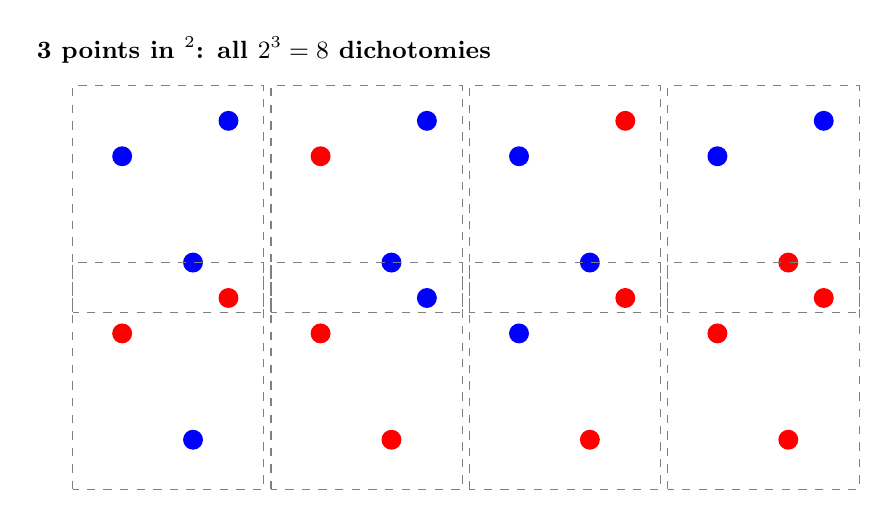
\begin{tikzpicture}[scale=0.9]
  % Shattering 3 points in R^2
  \node[font=\bfseries\small] at (2.5, 4.5) {3 points in $\R^2$: all $2^3=8$ dichotomies};
  \foreach \a/\b/\cc [count=\c from 0] in {
    0/0/0, 1/0/0, 0/1/0, 0/0/1,
    1/1/0, 1/0/1, 0/1/1, 1/1/1
  }{
    \pgfmathsetmacro{\col}{mod(\c,4)}
    \pgfmathsetmacro{\row}{int(\c/4)}
    \begin{scope}[shift={(\col*2.8, -\row*2.5)}]
      \ifnum\a=1
        \fill[red] (0.5,3) circle(4pt);
      \else
        \fill[blue] (0.5,3) circle(4pt);
      \fi
      \ifnum\b=1
        \fill[red] (2,3.5) circle(4pt);
      \else
        \fill[blue] (2,3.5) circle(4pt);
      \fi
      \ifnum\cc=1
        \fill[red] (1.5,1.5) circle(4pt);
      \else
        \fill[blue] (1.5,1.5) circle(4pt);
      \fi
      \draw[gray, dashed] (-0.2,0.8) rectangle (2.5,4);
    \end{scope}
  }
\end{tikzpicture}
\caption{A linear classifier in $\R^2$ can shatter 3 non-collinear points (all 8 labellings are realisable), so $\text{VC}(\mathcal{H})\geq 3$. One can show that no 4 points can be shattered, hence $\text{VC}=3=2+1$.}
\label{fig:vc-shattering}
\end{figure}

\begin{theorem}[VC Generalisation Bound]
For a hypothesis class $\mathcal{H}$ with $\text{VC}(\mathcal{H})=d<\infty$, with probability at least $1-\delta$ over an i.i.d.\ sample of size $n$:
\[
  R(\hat h) \leq \hat R(\hat h) + \sqrt{\frac{d\bigl(\ln(2n/d)+1\bigr)+\ln(4/\delta)}{n}}.
\]
\end{theorem}

\begin{remark}
The bound shows that generalisation is controlled by the ratio $d/n$. For reliable learning, we need $n\gg d$, i.e.\ far more samples than the VC dimension.
\end{remark}

%% ----------------------------------------------------------------
\section{The No Free Lunch Theorem}

\begin{theorem}[No Free Lunch (Wolpert, 1996)]
Averaged over \emph{all} possible target functions $f:\mathcal{X}\to\mathcal{Y}$ (uniformly), every learning algorithm has the same expected generalisation error. Formally, for any two algorithms $\mathcal{A}_1,\mathcal{A}_2$:
\[
  \sum_f \E_{\mathcal{D}\sim f}\bigl[R(\mathcal{A}_1(\mathcal{D}))\bigr]
  = \sum_f \E_{\mathcal{D}\sim f}\bigl[R(\mathcal{A}_2(\mathcal{D}))\bigr].
\]
\end{theorem}

\begin{remark}
The practical implication is that no algorithm is universally best. Domain knowledge and structural assumptions (inductive bias) are essential for good performance on any particular problem.
\end{remark}

%% ----------------------------------------------------------------
\section{Learning Curves}

\begin{definition}[Learning Curve]
A \emph{learning curve} plots the training and validation errors as functions of the training set size $n$. Characteristic patterns:
\begin{itemize}
  \item \textbf{High bias} (underfitting): both curves plateau at a high error; adding more data does not help.
  \item \textbf{High variance} (overfitting): large gap between training and validation error; more data helps.
\end{itemize}
\end{definition}

%% ----------------------------------------------------------------
\section{Implementation in Python}

\begin{codeblock}[title=\textbf{AIC/BIC for Polynomial Regression}]
\begin{minted}{python}
import numpy as np
import matplotlib.pyplot as plt

np.random.seed(42)
n = 50
X = np.sort(np.random.uniform(-3, 3, n))
y = np.sin(X) + 0.3 * np.random.randn(n)

aic_scores, bic_scores = [], []
degrees = range(1, 16)

for deg in degrees:
    # Fit polynomial
    Phi = np.vander(X, deg + 1, increasing=True)
    w = np.linalg.lstsq(Phi, y, rcond=None)[0]
    y_hat = Phi @ w
    residuals = y - y_hat
    sigma2 = np.sum(residuals**2) / n
    d = deg + 1  # number of parameters

    # Log-likelihood (Gaussian)
    log_lik = -n/2 * np.log(2*np.pi*sigma2) - n/2

    aic_scores.append(-2*log_lik + 2*d)
    bic_scores.append(-2*log_lik + d*np.log(n))

fig, ax = plt.subplots(figsize=(8, 5))
ax.plot(degrees, aic_scores, "bo-", label="AIC")
ax.plot(degrees, bic_scores, "rs-", label="BIC")
ax.set_xlabel("Polynomial Degree")
ax.set_ylabel("Information Criterion")
ax.legend(); ax.set_title("Model Selection via AIC and BIC")
plt.savefig("figures/ch11_aic_bic.pdf")
print(f"Best degree (AIC): {degrees[np.argmin(aic_scores)]}")
print(f"Best degree (BIC): {degrees[np.argmin(bic_scores)]}")
\end{minted}
\end{codeblock}

\begin{codeoutput}
\begin{verbatim}
Best degree (AIC): 4
Best degree (BIC): 3
\end{verbatim}
\end{codeoutput}

\begin{codeblock}[title=\textbf{Grid Search, Random Search, and Learning Curves}]
\begin{minted}{python}
from sklearn.datasets import load_digits
from sklearn.svm import SVC
from sklearn.model_selection import (
    GridSearchCV, RandomizedSearchCV, learning_curve
)
from scipy.stats import loguniform, randint
import matplotlib.pyplot as plt
import numpy as np

X, y = load_digits(return_X_y=True)

# Grid Search
param_grid = {"C": [0.1, 1, 10, 100], "gamma": [1e-3, 1e-4]}
gs = GridSearchCV(SVC(), param_grid, cv=5, scoring="accuracy")
gs.fit(X, y)
print(f"Grid search best: {gs.best_params_}, acc={gs.best_score_:.4f}")

# Random Search
param_dist = {"C": loguniform(0.01, 100), "gamma": loguniform(1e-5, 1e-1)}
rs = RandomizedSearchCV(SVC(), param_dist, n_iter=30, cv=5,
                         scoring="accuracy", random_state=42)
rs.fit(X, y)
print(f"Random search best: C={rs.best_params_['C']:.4f}, "
      f"gamma={rs.best_params_['gamma']:.6f}, acc={rs.best_score_:.4f}")

# Learning Curve
train_sizes, train_scores, val_scores = learning_curve(
    SVC(**rs.best_params_), X, y, cv=5,
    train_sizes=np.linspace(0.1, 1.0, 10), scoring="accuracy"
)

fig, ax = plt.subplots(figsize=(8, 5))
ax.plot(train_sizes, train_scores.mean(axis=1), "o-", label="Train")
ax.plot(train_sizes, val_scores.mean(axis=1), "s-", label="Validation")
ax.set_xlabel("Training Set Size"); ax.set_ylabel("Accuracy")
ax.legend(); ax.set_title("Learning Curve")
plt.savefig("figures/ch11_learning_curve.pdf")
\end{minted}
\end{codeblock}

\begin{codeblock}[title=\textbf{Bayesian Optimisation with Optuna}]
\begin{minted}{python}
import optuna
from sklearn.model_selection import cross_val_score
from sklearn.ensemble import GradientBoostingClassifier

optuna.logging.set_verbosity(optuna.logging.WARNING)

def objective(trial):
    params = {
        "n_estimators": trial.suggest_int("n_estimators", 50, 500),
        "max_depth": trial.suggest_int("max_depth", 2, 8),
        "learning_rate": trial.suggest_float("learning_rate", 0.01, 0.3,
                                              log=True),
        "subsample": trial.suggest_float("subsample", 0.6, 1.0),
    }
    clf = GradientBoostingClassifier(**params, random_state=42)
    return cross_val_score(clf, X, y, cv=5, scoring="accuracy").mean()

study = optuna.create_study(direction="maximize")
study.optimize(objective, n_trials=50)

print(f"Best accuracy: {study.best_value:.4f}")
print(f"Best params: {study.best_params}")
\end{minted}
\end{codeblock}

%% ----------------------------------------------------------------
\section{Exercises}

\begin{exercise}[AIC vs BIC]
Generate $n=100$ samples from $y=\sin(x)+\epsilon$, $\epsilon\sim\mathcal{N}(0,0.3^2)$. Fit polynomial models of degrees 1--20. Plot AIC and BIC as a function of degree. Which criterion selects a more parsimonious model? Repeat for $n=500$ and discuss.
\end{exercise}

\begin{exercise}[VC Dimension Computation]
Prove that the VC dimension of the class of intervals $h_{a,b}(x)=\ind\{a\leq x\leq b\}$ on $\R$ is exactly 2. \emph{Hint:} show that two points can be shattered, then show that no three points can.
\end{exercise}

\begin{exercise}[PAC Bound Application]
A hypothesis class has $|\mathcal{H}|=10^6$. How many samples $n$ are needed to guarantee that $R(\hat h)\leq\hat R(\hat h)+0.05$ with probability at least 0.95?
\end{exercise}

\begin{exercise}[Learning Curves Diagnosis]
Train a decision tree (no max depth) and a logistic regression on the digits dataset. Plot the learning curves for both. Identify which suffers from high bias and which from high variance. How could you improve each?
\end{exercise}

\begin{exercise}[Bayesian Optimisation]
Use Optuna (or scikit-optimize) to tune a random forest on the digits dataset over \texttt{n\_estimators}$\in[50,500]$, \texttt{max\_depth}$\in[3,20]$, \texttt{max\_features}$\in\{\text{sqrt, log2}\}$, and \texttt{min\_samples\_split}$\in[2,20]$. Compare the wall-clock time and best accuracy with grid search (coarse grid) and random search ($N=50$ iterations).
\end{exercise}

\begin{exercise}[No Free Lunch Interpretation]
Explain, in your own words, why the No Free Lunch theorem does not prevent practical machine learning from being useful. What role does inductive bias play?
\end{exercise}
